\documentclass{beamer}[10]
\usepackage{pgf}
\usepackage[danish]{babel}
\usepackage[utf8]{inputenc}
\usepackage{beamerthemesplit}
\usepackage{graphics,epsfig, subfigure}
\usepackage{url}
\usepackage{srcltx}
\usepackage{hyperref}
\usepackage{tikz}
\usepackage{moresize}
\usetikzlibrary{shapes.geometric, arrows}

\definecolor{kugreen}{RGB}{50,93,61}
\definecolor{kugreenlys}{RGB}{132,158,139}
\definecolor{kugreenlyslys}{RGB}{173,190,177}
\definecolor{kugreenlyslyslys}{RGB}{214,223,216}
\setbeamercovered{transparent}
\mode<presentation>
\usetheme[numbers,totalnumber,compress,sidebarshades]{PaloAlto}
\setbeamertemplate{footline}[frame number]

  \usecolortheme[named=kugreen]{structure}
  \useinnertheme{circles}
  \usefonttheme[onlymath]{serif}
  \setbeamercovered{transparent}
  \setbeamertemplate{blocks}[rounded][shadow=true]

\logo{\includegraphics[width=0.8cm]{KULogo}}
%\useoutertheme{infolines} 
\title{Image to text}
\author{Suraj Kiran S \\ Nakul A \\ Shinoj \\ Umesh U}
\institute{Government Engineering College, \\Sreekrishnapuram}
\date{} 



\begin{document}
\frame{\titlepage \vspace{-0.5cm}
}

\frame
{
\frametitle{Overview}
\tableofcontents%[pausesection]
}

\section{Literature survey}

\frame[allowframebreaks]{
\frametitle{Literature survey}
	\begin{itemize}
	\item Benjamin Z. Yao, Xiong Yang, Liang Lin, Mun Wai Lee and
Song-Chun Zhu proposed an image parsing to text
description that generates text for images and video content.
	\item Yi-Ren Yeh, Chun-Hao Huang, and
Yu-Chiang Frank Wang presents a novel domain adaptation
approach for solving cross domain pattern recognition
problem where data and features to be processed and
recognized are collected for different domains.
	\item S. Shahnawaz Ahmed, Shah Muhammed Abid Hussain and
Md. Sayeed Salam [8] introduced a model of image to text
conversion for electricity meter reading of units in kilo-watts
by capturing its image and sending that image in the form of
Multimedia Message Service (MMS) to the server.
	\item Fan-Chieh Cheng, Shih-Chia Huang, and Shanq-Jang
Ruan gave the technique of eliminating background model
form video sequence to detect foreground and objects;
	\item Iasonas Kokkinos and Petros Maragos formulate the
interaction between image segmentation and object
recognition using Expectation-Maximization (EM) algorithm.
	\end{itemize}
}


\section{Block diagram}

\frame{
\frametitle{Block diagram}
	\tikzstyle{box} = [rectangle, rounded corners, minimum width=3cm, minimum height=.5cm,text centered, draw=black, fill=red!30]
	\tikzstyle{square} = [rectangle, minimum width=3cm, minimum height=1cm, text centered, draw=black, fill=orange!30]
	\tikzstyle{arrow} = [thick,->,>=stealth]
	\begin{tikzpicture}[node distance=1.3cm]
	\node (1) [box] {Capture Image};
	\node (2) [box, right of=1,xshift=2cm] {Canny Transform};
	\node (3) [box, below of=2] {Skeletonization };
	\node (database) [square, right of=3,xshift=2.2cm,yshift=2.5cm] {Database };
	\node (4) [box, right of=3,xshift=2.2cm] {Machine Learning};
	\node (5) [box, below of=4] {Skeleton to text};
	\node (6) [box, below of=5] {Storage};
	\draw [arrow] (1) -- (2);
	\draw [arrow] (2) -- (3);
	\draw [arrow] (3) -- (4);
	\draw [arrow] (4) -- (5);
	\draw [arrow] (5) -- (6);
	\draw [arrow] (database) -- (4);
	
	\end{tikzpicture}
}
\section{Algorithms}

\frame{
\frametitle{Algorithms}
\begin{block}{}
\large \begin{center}
Algorithms
\end{center}
\end{block}
}

\subsection{Canny Transform}

\frame{
\frametitle{Canny Transform/Edge Detection}
	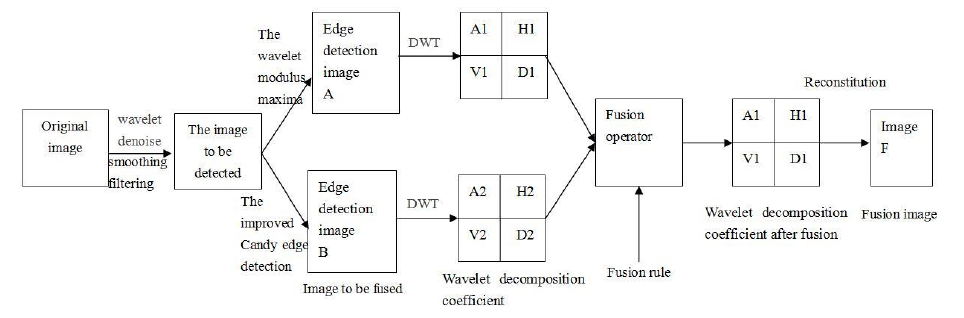
\includegraphics[scale=.3]{ct}
}

\subsection{Skeletonization}

\frame{
\frametitle{Skeletonization/Thinning}
jjjjjjjjj
}

\subsection{Machine Learning}

\frame{
\frametitle{Machine Learning}
			\begin{itemize}
			\item \textbf{Decision tree learning}
				\newline
				\begin{itemize}
					\item \scriptsize Uses a decision tree as a predictive model.
					\item Predictive modeling uses statistics to predict outcomes.
				\end{itemize}
			\end{itemize}
			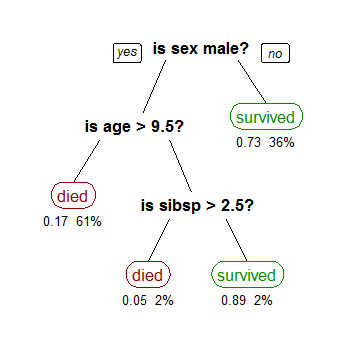
\includegraphics[scale=.4]{tree}
	}

\section{Execution}

\frame{
\frametitle{Implementation}
\begin{block}{}
\begin{center}
Execution
\end{center}
\end{block}
}
\subsection{Intitial setup}

\frame{
\frametitle{Intitial setup}
\begin{itemize}
	\item Install Android Studio
	\item Install Anaconda library
	\item Create new project Android studio
	\item Download and import OpenCV library to Android studio project
	\end{itemize}
}

\subsection{Tools}

\frame{
\frametitle{Tools}
	\begin{itemize}
	\item Android Studio
	\item Anaconda
	\item OpenCV
	\end{itemize}
}


\subsection{Dataset}

\frame{
\frametitle{Dataset}
	\begin{itemize}
	\item Skeleton of letters in the alphabet
	\item One to one maping of skeleton
	\end{itemize}
}




\end{document}
